\begin{abcliste}
\abc Jedes Wertepaar der Tabelle wird als Punkt eingetragen, mit der Zeit nach rechts und dem Ort nach oben (die Orte sind alle negativ). Weil die Ortsänderungen in je \SI{5}{\second} innerhalb der beiden Abschnitte gleich sind, liegen die Punkte auf zwei Geradenstücken:
\begin{center}
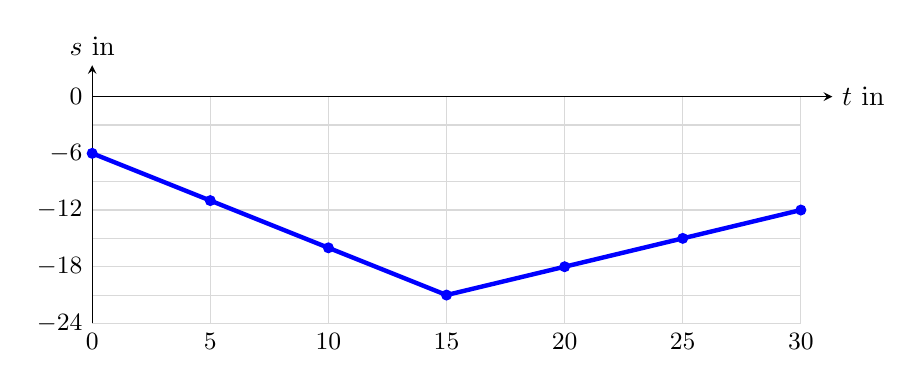
\begin{tikzpicture}[>=stealth, x=0.3cm, y=0.12cm]
 \draw[gray!30] (0,-24) grid[xstep=5, ystep=3] (30,0);
 \draw[->] (0,0) -- (31.333,0) node[right] {$t$ in \si{\second}};
 \draw[->] (0,-24) -- (0,3.333) node[above] {$s$ in \si{\meter}};
 \foreach \tk in {0,5,10,15,20,25,30} \node[below] at (\tk,-24) {\small $\tk$};
 \foreach \yk in {-24,-18,-12,-6,0} \node[left] at (0,\yk) {\small $\yk$};
 \draw[ultra thick, blue] (0,-6) -- (5,-11) -- (10,-16) -- (15,-21) -- (20,-18) -- (25,-15) -- (30,-12);
 \fill[blue] (0,-6) circle (2pt);
 \fill[blue] (5,-11) circle (2pt);
 \fill[blue] (10,-16) circle (2pt);
 \fill[blue] (15,-21) circle (2pt);
 \fill[blue] (20,-18) circle (2pt);
 \fill[blue] (25,-15) circle (2pt);
 \fill[blue] (30,-12) circle (2pt);
\end{tikzpicture}
\end{center}
Das ist $\result{\text{Diagramm (B)}}$.

\abc Bis \tMinO\ wird $s$ in jeweils \SI{5}{\second} um \SI{5}{\meter} kleiner: Das Fahrzeug fährt gleichförmig in die negative Richtung, mit
\begin{align}
 v_1 &= \vOneF = \frac{\sMin-\left(\sNull\right)}{\tMin} = \vOne \approx \result{\vOneP{0}{2}}
\end{align}
Danach wird $s$ in jeweils \SI{5}{\second} um \SI{3}{\meter} grösser: Das Fahrzeug fährt langsamer in die positive Richtung zurück, mit
\begin{align}
 v_2 &= \vTwoF = \frac{\sEnd-\left(\sMin\right)}{\tEnd-\tMin} = \vTwo \approx \result{\vTwoP{0}{2}}
\end{align}
Das Fahrzeug $\result{\text{kehrt bei } t\approx\tMinO \text{ um}}$, am Ort \sMinO, wo $s$ am kleinsten ist. Dass alle Orte negativ sind, spielt dabei keine Rolle: Die Fahrtrichtung zeigt sich daran, ob $s$ kleiner oder grösser wird, nicht am Vorzeichen von $s$.

\abc
\begin{itemize}
\item (A) ist zeitlich gespiegelt: Die Werte wurden von hinten nach vorne eingetragen (bei $t = 0$ steht der Wert von \SI{30}{\second}).
\item (B) ist richtig.
\item (C) zeigt nicht die Orte, sondern die Ortsänderungen $\Delta s$ in jedem \SI{5}{\second}-Abschnitt ($-5$, $-5$, $-5$, $+3$, $+3$, $+3$). Das ist (bis auf den Faktor $\SI{5}{\second}$) eher ein Geschwindigkeitsdiagramm.
\item (D) ist an der $t$-Achse gespiegelt: Die Minuszeichen wurden weggelassen. Das Fahrzeug würde dann zuerst in die positive Richtung fahren und danach zurück.
\end{itemize}
\end{abcliste}
